Najważniejszym krokiem całego procesu wykrywania logo \bk jest segmentacja. Celem procesu segmentacji jest automatyczne wydzielenie obszarów obrazu, których wygląd jest dla obserwatora spójny~\cite{pobr:wyklad}. Piksele spójne, to takie które spełniają podane kryterium jednorodności. Typowe kryteria jednorodności to podobny poziom jasności, podobny poziom barwy lub ta sama tekstura uzyskana w~wyniku analizy częstotliwościowej. Zasadniczo, proces segmentacji można podzielić na dwie fazy:
\begin{itemize}
    \item wydzielanie -- określenie czy dany piksel należy do interesującego obiektu czy też do tła,
    \item oznaczanie -- łączenie i~przyporządkowywanie interesujących pikseli do podzbiorów pikseli, będących potencjalnie obrazami szukanych obiektów.
\end{itemize}

Typowymi algorytmami segmentacji są algorytmy segmentacji przez progowanie, segmentacji krawędziowej, segmentacji metodą rozrostu obszarów, segmentacji metodą dziel i~łącz oraz metodą klasyfikacji punktów~\cite{pobr:wyklad}. Bardziej wyrafinowane metody segmentacji to m. in. segmentacja wododziałowa, segmentacja konturowa wykorzystująca uogólnioną transformatę Hougha oraz algorytm Random Sample Consensus (RanSaC)~\cite{perm:wyklad}.

W~przygotowanym rozwiązaniu wykorzystano algorytm hybrydowy, łączący ze sobą algorytm segmentacji przez progowanie oraz metodą rozrostu obszarów.

\subsubsection{Segmentacja przez progowanie - wydzielanie}
W~pierwszej kolejności, obraz został poddany działania algorytmu segmentacji przez progowanie. Celem tego kroku było wydzielenie elementów logo \bk oraz odfiltrowanie pikseli nienależących do poszukiwanego znaku graficznego. W~tym celu, obrabiany obraz został powielony czterokrotnie, a~następnie każda z~kopii została poddana prostemu progowaniu. Każda z~kopii odpowiada jednej barwie w~poszukiwanym logo, tj. czerwonej, niebieskiej, białej oraz żółtej.

Z~każdym progowaniem, związany jest obiekt typu \texttt{POBR::HSVMask}. Obiekt ten przechowuje 6 parametrów:
\begin{itemize}
    \item minimalna wartość \emph{Hue} $H_{\mathrm{min}}$,
    \item maksymalna wartość \emph{Hue} $H_{\mathrm{min}}$,
    \item minimalna wartość \emph{Saturation} $S_{\mathrm{min}}$,
    \item maksymalna wartość \emph{Saturation} $S_{\mathrm{max}}$,
    \item minimalna wartość \emph{Value} $V_{\mathrm{min}}$,
    \item maksymalna wartość \emph{Value} $V_{\mathrm{max}}$.
\end{itemize}

Dla każdego piksela $P_{ij} = (H_{ij}, S_{ij}, V_{ij})$, obiekt ten sprawdza  nierówności~\ref{eqn:hsvmask}.

\begin{equation}
    \begin{aligned}
        H_{\mathrm{min}} \leq H_{ij} \leq H_{\mathrm{max}} \\
        S_{\mathrm{min}} \leq S_{ij} \leq S_{\mathrm{max}} \\
        V_{\mathrm{min}} \leq V_{ij} \leq V_{\mathrm{max}}
    \end{aligned}
    \label{eqn:hsvmask}
\end{equation}

Niespełnienie chociażby jednej z~nierówności~\ref{eqn:hsvmask} powoduje odrzucenie danego piksela. Każda z~czterech kopii obrazu oryginalnego jest analizowana osobno, ze względu na przypisany kolor. Wartości zastosowanych progów zostały przedstawione w~tabeli poniżej.

\begin{center}
\begin{tabular}{c|c|c|c|c|c|c}
    Kolor & $H_{\mathrm{min}}$ & $H_{\mathrm{max}}$ & $S_{\mathrm{min}}$ & $S_{\mathrm{max}}$ & $V_{\mathrm{min}}$ & $V_{\mathrm{max}}$ \\ \hline 
    czerwony & $-20\degree$ & $20\degree$ & $150$ & $255$ & $100$ & $255$ \\ \hline
    niebieski & $ 220\degree$ & $300\degree$ & $70$ & $255$ & $0$ & $255$ \\ \hline
    biały & $0\degree$ & $360\degree$ & $0$ & $75$ & $100$ & $255$ \\ \hline
    żółty & $20\degree$ & $60\degree$ & $80$ & $255$ & $150$ & $255$ 
\end{tabular}
\end{center}

Rezultatem tak przeprowadzonego progowania jest binarna macierz gdzie $0$~oznacza że piksel nie spełnia nierówności, natomiast~$1$ że piksel spełnia wszystkie nierówności. 

Dla niektórych kolorów, macierz ta zostaje dodatkowo poddana działaniu filtrów rankingowych: minimum i~maksimum, w~celu wykonania morfologicznej operacji erozji i~dylatacji. Złożenie tych operacji pozwala na wykonanie operacji otwarcia i~domknięcia obrazu. 

Ostatnim krokiem wydzielania, jest połączenie uzyskanych czterech binarnych macierzy w~jedną typu \texttt{cv::Mat\_{}<POBR::Color>}, gdzie typ \texttt{POBR::Color} to typ wyliczeniowy, który opisuje pięć różnych kolorów (\texttt{RED, BLUE, WHITE, YELLOW OTHER}). 

\subsubsection{Segmentacja metodą rozrostu obszarów - oznaczanie}
Przygotowana macierz kolorów pozwala na przeprowadzenie rozrostu obszarów. Celem tej metody jest uzyskanie odrębnych grup pikseli -- segmentów. W~programie, segment obrazu jest reprezentowany jako lista pozycji $(y, x)$ pikseli należących do tego segmentu.

\begin{figure}[tb]
    \centering
    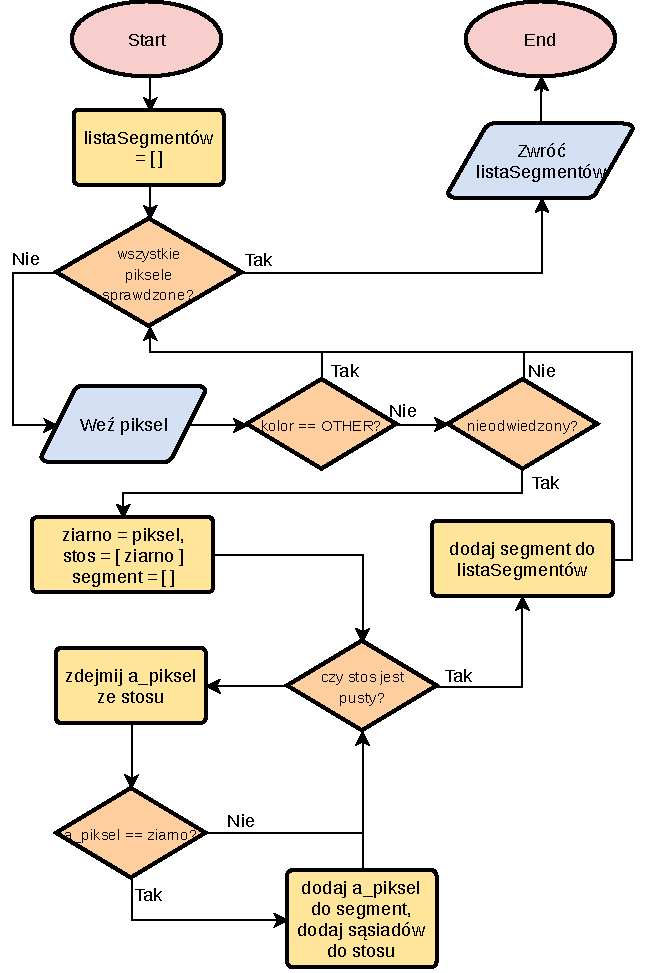
\includegraphics[width=\columnwidth]{figures/POBR-Segmentation.pdf}
    \caption{Ogólny schemat blokowy algorytmu segmentacji metodą rozrostu obszarów}
    \label{fig:segmentation-overview}
\end{figure}

W~metodzie oprócz macierzy kolorów, wykorzystywana jest również macierz stanów pikseli. Piksel może mieć jeden z~czterech stanów: \emph{nieodwiedzony}, \emph{sprawdzony}, \emph{dodany}, \emph{pominięty}.Przed uruchomieniem algorytmu, wszystkie komórki macierzy stanów są inicjalizowane stanem \emph{nieodwiedzony}.


Na rysunku~\ref{fig:segmentation-overview} przedstawiony został schemat blokowy algorytmu segmentacji metodą rozrostu obszarów. Algorytm iterując po kolei po wszystkich pikselach szuka nieodwiedzonych pikseli, których kolor jest inny niż \texttt{OTHER}. Jeżeli taki znajdzie, przyjmuje go za ziarno i~rozpoczyna budowę segmentu.

Do budowy segmentu wykorzystany został stos, na którym znajdują się przetwarzane piksele. Po umieszczeniu ziarna na stosie, algorytm iteruje do momentu aż stos będzie pusty, sprawdzając piksel który znajduje się na szczycie stosu. Jeżeli piksel ten jest taki sam jak ziarno, to zostaje on włączony do segmentu, a na stos wrzucane są piksele sąsiadujące z~nim. Algorytm kończy pracę gdy nie będzie już żadnego piksela ze stanem \emph{nieodwiedzony}.

Przedstawiony algorytm różni się trochę od oryginalnej wersji algorytmu, w~której ziarna dobierane są losowo przed iterowaniem po obrazie. Zaprezentowana wersja pozwala na jednoznaczne wyznaczenie segmentów, bez obawy że część segmentów nie zostanie odnaleziona z~powodu złego dobrania ziaren początkowych, kosztem większej złożoności obliczeniowej.

Algorytm ten posiada jeszcze jedną wadę, mianowicie wychwytuje bardzo dużo małych segmentów zawierających po kilka pikseli. W~tym celu, po wyznaczaniu segmentów, algorytm sortuje wszystkie piksele według ich rozmiaru i~odfiltrowuje wszystkie segmenty, których rozmiar jest mniejszy niż podany próg.
